% Options for packages loaded elsewhere
\PassOptionsToPackage{unicode}{hyperref}
\PassOptionsToPackage{hyphens}{url}
%
\documentclass[
]{article}
\usepackage{amsmath,amssymb}
\usepackage{lmodern}
\usepackage{iftex}
\ifPDFTeX
  \usepackage[T1]{fontenc}
  \usepackage[utf8]{inputenc}
  \usepackage{textcomp} % provide euro and other symbols
\else % if luatex or xetex
  \usepackage{unicode-math}
  \defaultfontfeatures{Scale=MatchLowercase}
  \defaultfontfeatures[\rmfamily]{Ligatures=TeX,Scale=1}
\fi
% Use upquote if available, for straight quotes in verbatim environments
\IfFileExists{upquote.sty}{\usepackage{upquote}}{}
\IfFileExists{microtype.sty}{% use microtype if available
  \usepackage[]{microtype}
  \UseMicrotypeSet[protrusion]{basicmath} % disable protrusion for tt fonts
}{}
\makeatletter
\@ifundefined{KOMAClassName}{% if non-KOMA class
  \IfFileExists{parskip.sty}{%
    \usepackage{parskip}
  }{% else
    \setlength{\parindent}{0pt}
    \setlength{\parskip}{6pt plus 2pt minus 1pt}}
}{% if KOMA class
  \KOMAoptions{parskip=half}}
\makeatother
\usepackage{xcolor}
\usepackage[margin=1in]{geometry}
\usepackage{color}
\usepackage{fancyvrb}
\newcommand{\VerbBar}{|}
\newcommand{\VERB}{\Verb[commandchars=\\\{\}]}
\DefineVerbatimEnvironment{Highlighting}{Verbatim}{commandchars=\\\{\}}
% Add ',fontsize=\small' for more characters per line
\usepackage{framed}
\definecolor{shadecolor}{RGB}{248,248,248}
\newenvironment{Shaded}{\begin{snugshade}}{\end{snugshade}}
\newcommand{\AlertTok}[1]{\textcolor[rgb]{0.94,0.16,0.16}{#1}}
\newcommand{\AnnotationTok}[1]{\textcolor[rgb]{0.56,0.35,0.01}{\textbf{\textit{#1}}}}
\newcommand{\AttributeTok}[1]{\textcolor[rgb]{0.77,0.63,0.00}{#1}}
\newcommand{\BaseNTok}[1]{\textcolor[rgb]{0.00,0.00,0.81}{#1}}
\newcommand{\BuiltInTok}[1]{#1}
\newcommand{\CharTok}[1]{\textcolor[rgb]{0.31,0.60,0.02}{#1}}
\newcommand{\CommentTok}[1]{\textcolor[rgb]{0.56,0.35,0.01}{\textit{#1}}}
\newcommand{\CommentVarTok}[1]{\textcolor[rgb]{0.56,0.35,0.01}{\textbf{\textit{#1}}}}
\newcommand{\ConstantTok}[1]{\textcolor[rgb]{0.00,0.00,0.00}{#1}}
\newcommand{\ControlFlowTok}[1]{\textcolor[rgb]{0.13,0.29,0.53}{\textbf{#1}}}
\newcommand{\DataTypeTok}[1]{\textcolor[rgb]{0.13,0.29,0.53}{#1}}
\newcommand{\DecValTok}[1]{\textcolor[rgb]{0.00,0.00,0.81}{#1}}
\newcommand{\DocumentationTok}[1]{\textcolor[rgb]{0.56,0.35,0.01}{\textbf{\textit{#1}}}}
\newcommand{\ErrorTok}[1]{\textcolor[rgb]{0.64,0.00,0.00}{\textbf{#1}}}
\newcommand{\ExtensionTok}[1]{#1}
\newcommand{\FloatTok}[1]{\textcolor[rgb]{0.00,0.00,0.81}{#1}}
\newcommand{\FunctionTok}[1]{\textcolor[rgb]{0.00,0.00,0.00}{#1}}
\newcommand{\ImportTok}[1]{#1}
\newcommand{\InformationTok}[1]{\textcolor[rgb]{0.56,0.35,0.01}{\textbf{\textit{#1}}}}
\newcommand{\KeywordTok}[1]{\textcolor[rgb]{0.13,0.29,0.53}{\textbf{#1}}}
\newcommand{\NormalTok}[1]{#1}
\newcommand{\OperatorTok}[1]{\textcolor[rgb]{0.81,0.36,0.00}{\textbf{#1}}}
\newcommand{\OtherTok}[1]{\textcolor[rgb]{0.56,0.35,0.01}{#1}}
\newcommand{\PreprocessorTok}[1]{\textcolor[rgb]{0.56,0.35,0.01}{\textit{#1}}}
\newcommand{\RegionMarkerTok}[1]{#1}
\newcommand{\SpecialCharTok}[1]{\textcolor[rgb]{0.00,0.00,0.00}{#1}}
\newcommand{\SpecialStringTok}[1]{\textcolor[rgb]{0.31,0.60,0.02}{#1}}
\newcommand{\StringTok}[1]{\textcolor[rgb]{0.31,0.60,0.02}{#1}}
\newcommand{\VariableTok}[1]{\textcolor[rgb]{0.00,0.00,0.00}{#1}}
\newcommand{\VerbatimStringTok}[1]{\textcolor[rgb]{0.31,0.60,0.02}{#1}}
\newcommand{\WarningTok}[1]{\textcolor[rgb]{0.56,0.35,0.01}{\textbf{\textit{#1}}}}
\usepackage{graphicx}
\makeatletter
\def\maxwidth{\ifdim\Gin@nat@width>\linewidth\linewidth\else\Gin@nat@width\fi}
\def\maxheight{\ifdim\Gin@nat@height>\textheight\textheight\else\Gin@nat@height\fi}
\makeatother
% Scale images if necessary, so that they will not overflow the page
% margins by default, and it is still possible to overwrite the defaults
% using explicit options in \includegraphics[width, height, ...]{}
\setkeys{Gin}{width=\maxwidth,height=\maxheight,keepaspectratio}
% Set default figure placement to htbp
\makeatletter
\def\fps@figure{htbp}
\makeatother
\setlength{\emergencystretch}{3em} % prevent overfull lines
\providecommand{\tightlist}{%
  \setlength{\itemsep}{0pt}\setlength{\parskip}{0pt}}
\setcounter{secnumdepth}{-\maxdimen} % remove section numbering
\ifLuaTeX
  \usepackage{selnolig}  % disable illegal ligatures
\fi
\IfFileExists{bookmark.sty}{\usepackage{bookmark}}{\usepackage{hyperref}}
\IfFileExists{xurl.sty}{\usepackage{xurl}}{} % add URL line breaks if available
\urlstyle{same} % disable monospaced font for URLs
\hypersetup{
  pdftitle={The Thickness of Collagen Membrane},
  pdfauthor={Frank (Bo-Jiang Lin)},
  hidelinks,
  pdfcreator={LaTeX via pandoc}}

\title{The Thickness of Collagen Membrane}
\author{Frank (Bo-Jiang Lin)}
\date{2022-08-28}

\begin{document}
\maketitle

\hypertarget{github-documents}{%
\subsection{GitHub Documents}\label{github-documents}}

This is an R Markdown format used for publishing markdown documents to
GitHub. When you click the \textbf{Knit} button all R code chunks are
run and a markdown file (.md) suitable for publishing to GitHub is
generated.

\hypertarget{including-code}{%
\subsection{Including Code}\label{including-code}}

\hypertarget{configure-the-necessary-environment-and-packages}{%
\subsubsection{1. Configure the necessary environment and
packages}\label{configure-the-necessary-environment-and-packages}}

\begin{Shaded}
\begin{Highlighting}[]
\NormalTok{version[[}\StringTok{\textquotesingle{}version.string\textquotesingle{}}\NormalTok{]]}
\end{Highlighting}
\end{Shaded}

\begin{verbatim}
## [1] "R version 4.2.1 (2022-06-23 ucrt)"
\end{verbatim}

\begin{Shaded}
\begin{Highlighting}[]
\FunctionTok{library}\NormalTok{(readxl)}
\FunctionTok{library}\NormalTok{(UsingR)}
\end{Highlighting}
\end{Shaded}

\begin{verbatim}
## Loading required package: MASS
\end{verbatim}

\begin{verbatim}
## Loading required package: HistData
\end{verbatim}

\begin{verbatim}
## Loading required package: Hmisc
\end{verbatim}

\begin{verbatim}
## Loading required package: lattice
\end{verbatim}

\begin{verbatim}
## Loading required package: survival
\end{verbatim}

\begin{verbatim}
## Loading required package: Formula
\end{verbatim}

\begin{verbatim}
## Loading required package: ggplot2
\end{verbatim}

\begin{verbatim}
## 
## Attaching package: 'Hmisc'
\end{verbatim}

\begin{verbatim}
## The following objects are masked from 'package:base':
## 
##     format.pval, units
\end{verbatim}

\begin{verbatim}
## 
## Attaching package: 'UsingR'
\end{verbatim}

\begin{verbatim}
## The following object is masked from 'package:survival':
## 
##     cancer
\end{verbatim}

\begin{Shaded}
\begin{Highlighting}[]
\FunctionTok{library}\NormalTok{(lessR)}
\end{Highlighting}
\end{Shaded}

\begin{verbatim}
## 
## lessR 4.2.2                         feedback: gerbing@pdx.edu 
## --------------------------------------------------------------
## > d <- Read("")   Read text, Excel, SPSS, SAS, or R data file
##   d is default data frame, data= in analysis routines optional
## 
## Learn about reading, writing, and manipulating data, graphics,
## testing means and proportions, regression, factor analysis,
## customization, and descriptive statistics from pivot tables.
##   Enter:  browseVignettes("lessR")
## 
## View changes in this or recent versions of lessR.
##   Enter: help(package=lessR)  Click: Package NEWS
##   Enter: interact()  for access to interactive graphics
##   New function: reshape_long() to move data from wide to long
\end{verbatim}

\begin{verbatim}
## 
## Attaching package: 'lessR'
\end{verbatim}

\begin{verbatim}
## The following objects are masked from 'package:Hmisc':
## 
##     label, Merge
\end{verbatim}

\begin{Shaded}
\begin{Highlighting}[]
\FunctionTok{library}\NormalTok{(ggplot2)}
\end{Highlighting}
\end{Shaded}

\hypertarget{read-data}{%
\subsubsection{2. Read Data}\label{read-data}}

\begin{verbatim}
## # A tibble: 5 x 14
##   Date       Person 60 mm Dish~1 Buffe~2 Total~3 Centr~4 Uncom~5 7days~6 0 day~7
##   <date>     <chr>         <dbl>   <dbl>   <dbl>   <dbl>   <dbl>   <dbl>   <dbl>
## 1 2022-08-28 Frank         6262.      NA      NA      NA      NA      NA      NA
## 2 2022-08-28 Frank         6253.      NA      NA      NA      NA      NA      NA
## 3 2022-08-28 Frank         6248.      NA      NA      NA      NA      NA      NA
## 4 2022-08-28 Frank         6268.      NA      NA      NA      NA      NA      NA
## 5 2022-08-28 Frank         6263.      NA      NA      NA      NA      NA      NA
## # ... with 5 more variables: `Compressed Thickness  (μm) after 7 days` <dbl>,
## #   `Compressed Thickness  (μm) after 0 days` <dbl>,
## #   UnCompressed_Thickness <dbl>, `7days Compression ratio` <dbl>,
## #   `0 days Compression ratio` <dbl>, and abbreviated variable names
## #   1: `60 mm Dish (μm)`, 2: `Buffer (pH)`, 3: Total_solution_quantity,
## #   4: `Centrifuge time (min)`, 5: `Uncompressed Depth (μm)`,
## #   6: `7days and Compressed Depth (μm)`, ...
\end{verbatim}

\hypertarget{exploratory-data-analysis-for-2022-08-28-data}{%
\subsubsection{3. Exploratory Data Analysis for 2022-08-28
data}\label{exploratory-data-analysis-for-2022-08-28-data}}

\hypertarget{descriptive-statistics-on-the-2022-08-28-data}{%
\paragraph{Descriptive Statistics on the 2022-08-28
data}\label{descriptive-statistics-on-the-2022-08-28-data}}

\begin{verbatim}
##   Group.1 Total_solution_quantity UnCompressed_Thickness
## 1     1.0                     1.0               471.7582
## 2     1.5                     1.5               627.5724
\end{verbatim}

\hypertarget{check-whether-the-2022-08-28-data-is-normal-distribution}{%
\paragraph{Check whether the 2022-08-28 data is normal
distribution}\label{check-whether-the-2022-08-28-data-is-normal-distribution}}

\begin{Shaded}
\begin{Highlighting}[]
\FunctionTok{summary}\NormalTok{(collagen}\SpecialCharTok{$}\NormalTok{UnCompressed\_Thickness)}
\end{Highlighting}
\end{Shaded}

\begin{verbatim}
##    Min. 1st Qu.  Median    Mean 3rd Qu.    Max.    NA's 
##   331.1   447.3   511.6   519.6   551.4   816.3      15
\end{verbatim}

\begin{Shaded}
\begin{Highlighting}[]
\CommentTok{\#Creat a table}

\NormalTok{normal }\OtherTok{\textless{}{-}} \FunctionTok{shapiro.test}\NormalTok{(collagen}\SpecialCharTok{$}\NormalTok{UnCompressed\_Thickness)}
\NormalTok{normal}
\end{Highlighting}
\end{Shaded}

\begin{verbatim}
## 
##  Shapiro-Wilk normality test
## 
## data:  collagen$UnCompressed_Thickness
## W = 0.94094, p-value = 0.1556
\end{verbatim}

\hypertarget{the-2022-08-28-data-shows-p-value-0.16-0.1.-it-represent-that-the-data-distrubute-normally-and-ready-for-further-test..}{%
\subparagraph{The 2022-08-28 data shows p-value = 0.16 \textgreater=
0.1. It represent that the data distrubute normally and ready for
further
test..}\label{the-2022-08-28-data-shows-p-value-0.16-0.1.-it-represent-that-the-data-distrubute-normally-and-ready-for-further-test..}}

\begin{Shaded}
\begin{Highlighting}[]
\NormalTok{comparison }\OtherTok{\textless{}{-}} \FunctionTok{t.test}\NormalTok{(collagen\_Frank}\SpecialCharTok{$}\NormalTok{UnCompressed\_Thickness }\SpecialCharTok{\textasciitilde{}}\NormalTok{ collagen\_Frank}\SpecialCharTok{$}\NormalTok{Total\_solution\_quantity)}
\NormalTok{comparison}
\end{Highlighting}
\end{Shaded}

\begin{verbatim}
## 
##  Welch Two Sample t-test
## 
## data:  collagen_Frank$UnCompressed_Thickness by collagen_Frank$Total_solution_quantity
## t = -1.937, df = 5.7962, p-value = 0.1026
## alternative hypothesis: true difference in means between group 1 and group 1.5 is not equal to 0
## 95 percent confidence interval:
##  -354.33488   42.70648
## sample estimates:
##   mean in group 1 mean in group 1.5 
##          471.7582          627.5724
\end{verbatim}

\hypertarget{the-2022-08-28-data-shows-p-value-is-0.1-0.05-which-means-we-accept-the-h0-hypothesis.}{%
\subparagraph{The 2022-08-28 data shows p-value is 0.1 \textgreater=
0.05 which means we accept the H0
hypothesis.}\label{the-2022-08-28-data-shows-p-value-is-0.1-0.05-which-means-we-accept-the-h0-hypothesis.}}

\hypertarget{reproducibility}{%
\subsubsection{4. Reproducibility}\label{reproducibility}}

\begin{verbatim}
##      Group.1 Total_solution_quantity UnCompressed_Thickness
## 1      Frank                       1               471.7582
## 2 沢崎ちゃん                       1               499.5648
\end{verbatim}

\begin{Shaded}
\begin{Highlighting}[]
\NormalTok{reproducibility }\OtherTok{\textless{}{-}} \FunctionTok{t.test}\NormalTok{(collagen\_1ml}\SpecialCharTok{$}\NormalTok{UnCompressed\_Thickness }\SpecialCharTok{\textasciitilde{}}\NormalTok{ collagen\_1ml}\SpecialCharTok{$}\NormalTok{Person)}
\NormalTok{reproducibility}
\end{Highlighting}
\end{Shaded}

\begin{verbatim}
## 
##  Welch Two Sample t-test
## 
## data:  collagen_1ml$UnCompressed_Thickness by collagen_1ml$Person
## t = -0.69612, df = 6.4676, p-value = 0.5106
## alternative hypothesis: true difference in means between group Frank and group 沢崎ちゃん is not equal to 0
## 95 percent confidence interval:
##  -123.86058   68.24741
## sample estimates:
##      mean in group Frank mean in group 沢崎ちゃん 
##                 471.7582                 499.5648
\end{verbatim}

\hypertarget{the-p-value-is-0.51-which-means-the-data-reach-to-the-consensus-results-while-p-value-is-higher-than-0.05.}{%
\subparagraph{The p-value is 0.51 which means the data reach to the
consensus results while p-value is higher than
0.05.}\label{the-p-value-is-0.51-which-means-the-data-reach-to-the-consensus-results-while-p-value-is-higher-than-0.05.}}

\hypertarget{including-plots}{%
\subsection{Including Plots}\label{including-plots}}

\hypertarget{the-distribution-of-the-2022-08-28-data}{%
\subsubsection{1. the distribution of the 2022-08-28
data}\label{the-distribution-of-the-2022-08-28-data}}

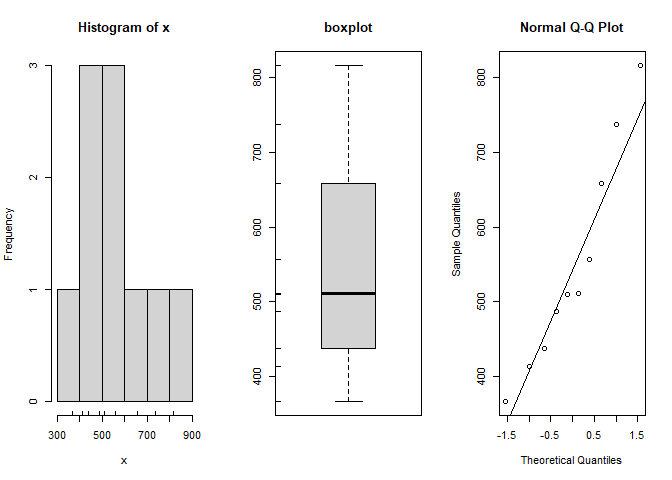
\includegraphics{Collagen-Membrane_files/figure-latex/normal plot-1.pdf}

\hypertarget{the-comparison-of-the-2022-08-28-data}{%
\subsubsection{2. the comparison of the 2022-08-28
data}\label{the-comparison-of-the-2022-08-28-data}}

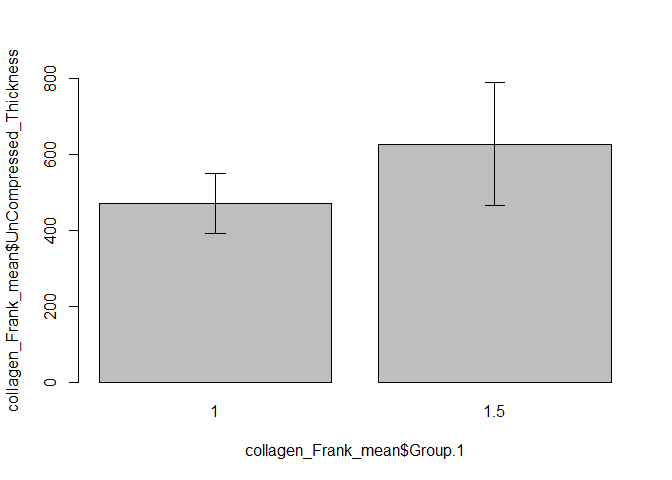
\includegraphics{Collagen-Membrane_files/figure-latex/comparison-1.pdf}

\hypertarget{the-comparison-study-on-the-2022-08-28-data-with-the-prvious-study}{%
\subsubsection{3. the comparison study on the 2022-08-28 data with the
prvious
study}\label{the-comparison-study-on-the-2022-08-28-data-with-the-prvious-study}}

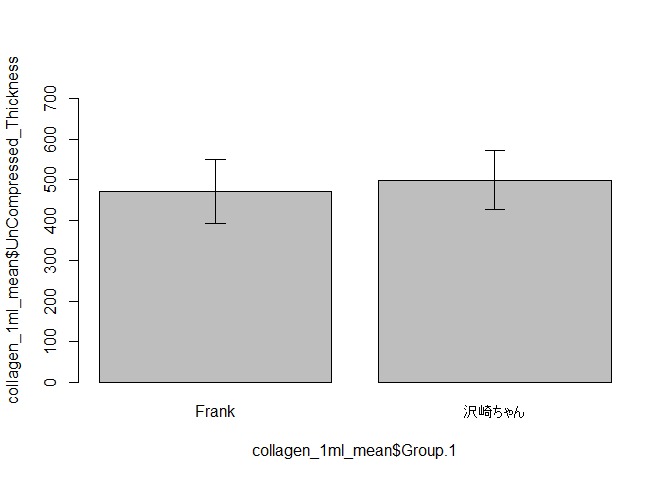
\includegraphics{Collagen-Membrane_files/figure-latex/reproducibility-1.pdf}

Note that the \texttt{echo\ =\ FALSE} parameter was added to the code
chunk to prevent printing of the R code that generated the plot.

\end{document}
